\documentclass[12pt]{article}
\usepackage{graphicx}
\usepackage[toc,page]{appendix}
\usepackage{cite}
\graphicspath{ {images/} }
\usepackage{listings}

\usepackage{enumitem}


\lstset{numbers=left}

\begin{document}

\begin{titlepage}

\newcommand{\HRule}{\rule{\linewidth}{0.5mm}} % Defines a new command for the horizontal lines, change thickness here

\center % Center everything on the page
 
%----------------------------------------------------------------------------------------
%	HEADING SECTIONS
%----------------------------------------------------------------------------------------

\textsc{\LARGE Queensland University of Technology}\\[1.5cm] % Name of your university/college
\textsc{\Large CAB432}\\[0.5cm] % Major heading such as course name
\textsc{\large Assignment 1}\\[0.5cm] % Minor heading such as course title

%----------------------------------------------------------------------------------------
%	TITLE SECTION
%----------------------------------------------------------------------------------------

\HRule \\[0.4cm]
{ \huge \bfseries Docker Mashup Project }\\[0.4cm] % Title of your document
\HRule \\[1.5cm]
 
%----------------------------------------------------------------------------------------
%	AUTHOR SECTION
%----------------------------------------------------------------------------------------

\begin{minipage}{0.4\textwidth}
\begin{flushleft} \large
\emph{Author:}\\
Joshua Miles[n7176244] % Your name
\end{flushleft}
\end{minipage}
~
\begin{minipage}{0.4\textwidth}
\begin{flushright} \large
\emph{Tutor:} \\
 \textsc{} % Supervisor's Name
\end{flushright}
\end{minipage}\\[0.5cm]

% If you don't want a supervisor, uncomment the two lines below and remove the section above
%\Large \emph{Author:}\\
%John \textsc{Smith}\\[3cm] % Your name

%----------------------------------------------------------------------------------------
%	DATE SECTION
%----------------------------------------------------------------------------------------

{\large 22$^{nd}$ April 2016}\\[2cm] % Date, change the \today to a set date if you want to be precise

%----------------------------------------------------------------------------------------
%	LOGO SECTION
%----------------------------------------------------------------------------------------


\includegraphics[scale=0.10]{qut-logo-better}\\[2cm] % Include a department/university logo - this will require the graphicx package
 
%----------------------------------------------------------------------------------------

% \vfill % Fill the rest of the page with whitespace

\end{titlepage}

%----------------------------------------------------------------------------------------


\tableofcontents
\newpage




\section{Introduction}
 mashup purpose and description (updated as needed from the proposal). This should include an introductory section, outlining the overall purpose and some idea of the sorts of usages supported, but described informally (this is probably 3 or 4 paragraphs). You should then have a description of the services used, with URL and one paragraph description of each. Don’t get to the deep API level here.
 
 

\section{  }
Mashup use cases and services – this section should outline explicitly the use cases supported by the mashup (these must be illustrated using screen shots) and the service API calls used to support them. This is a semi-technical description, probably
occupying about a page per use case.
\subsection{}

\subsubsection{Basic Operations}


\subsubsection{System Time}


%the same as average case efficency
\subsection{Order of Growth}
 The expected order of growth is $\Theta(n^2)$ as Knuth\cite[p.80]{knuth1998art} and Cormen et al \cite[p.26]{cormen2009linear} noted. This is also affirmed in the above section as it is the dominant factor in the Average Case efficiency for both the count of basic operation and the system time. Thus, if the Average Case efficiency turns out to be $\frac{n^2}{4}$ it is assumed that the $\frac{n^2}{4}	\in\Theta(n^2)$ is true.


\section{Theoretical Analysis of the Algorithm}

\subsection{Characteristics}




\subsection{Input}

\section{Technical Description}

Technical description of the application. This is a deeper discussion of the architecture,
the technology used on the client and server side, any issues encountered, and overall,
how you implemented the project.

\subsection{The Code}

\section{Discussion of the use of Docker}


\section{Testing and limitations} 


\section{Extensions}

\subsubsection{Writing to CSV}


\subsubsection{Finding the Average and Graphing}

\begin{itemize}[noitemsep]

\end{itemize}

\subsection{Tools}


\section{Results}

\subsection{Average Time}

\subsection{Average Number of Basic Operations}

\subsection{Comparison}

\section{Conclusion}

\bibliography{bib/tex}
%\bibliographystyle{IEEE}

\newpage


\begin{appendices}
\section{The Insertion Sort Algorithm}
\begin{figure}[h]
\begin{lstlisting}
ALGORITHM InsertionSort(A[0...n-1])
	for i <- to n-1 do
		v <- A[i]
		j <- i - 1
		while j >= 0 and A[j] > v do
			A[j+1] <- A[j]
			j <- j-1
	A[j+1] <-v
\end{lstlisting}
\caption{\label{the-algorithm-psuedo} The inefficient pseudo code for the Insertion Sort algorithm}
\end{figure}

\newpage	

\section{Coded Algorithm using Basic Operations}
\label{coded-algo-basic}
\begin{figure}[h]
\begin{lstlisting}[language=C++, breaklines=true]
int *InsertionSortBasicOperations(int *unsortedArray, int lengthOfUnsortedArray) {
	int j, temp;
	basicOperations = 0;
	for (int i = 1; i <= lengthOfUnsortedArray-1; ++i) {
		temp = unsortedArray[i];
		j = i-1;
		while (j >= 0 && unsortedArray[j]>temp){
			unsortedArray[j+1] = unsortedArray[j];
			j--;
			basicOperations++;
		};
	unsortedArray[j+1] = temp;
	}

	return unsortedArray;
}
\end{lstlisting}
\caption{\label{insertion-sort-basic} The insertion sort algorithm in the language C++ which includes the basic operation}
\end{figure}

\newpage
\section{Coded Algorithm using System Time}
%\label{}
\begin{figure}[h]
\begin{lstlisting}[language=C++, breaklines=true]
int *InsertionSortTime(int *unsortedArray, int lengthOfUnsortedArray) {
	int j, temp;
	for (int i = 1; i <= lengthOfUnsortedArray-1; ++i) {
		temp = unsortedArray[i];
		j = i-1;
		while (j >= 0 && unsortedArray[j]>temp){
			unsortedArray[j+1] = unsortedArray[j];
			j--;
		};
		unsortedArray[j+1] = temp;
	}
	return unsortedArray;
}
\end{lstlisting}
\caption{\label{coded-algo-time} The insertion sort algorithm in the language C++ which doesn't include the basic operation}
\end{figure}
\newpage

\section{Running the Algorithm while Timed}
\begin{figure}[h]
\begin{lstlisting}
double performAlgorithmAndTime(int sizeOfInput) {
	int *randomArray = makeDataRandom(sizeOfInput);
	start = std::clock();
	InsertionSortTime(randomArray, sizeOfInput);
	duration = (clock() - start) / (double) CLOCKS_PER_SEC;
	return duration;
};
\end{lstlisting}
\caption{\label{perform-algo-and-time} This function uses the C++ language to start a clock, perform an algorithm and than find out the time between the start time and the current time.}
\end{figure}
\newpage

\section{Building the random Data}
\begin{figure}[h]
\begin{lstlisting}[language=C++, breaklines=true]
int* makeDataRandom(int lengthOfArray) {
	int *arr = new int[lengthOfArray],v1;
	for (int i = 0; i < lengthOfArray; ++i) {
		v1 = rand() % 1000000;
		arr[i] = v1;
	}
	return arr;
}
\end{lstlisting}
\caption{\label{make-data-random}The C++ code related to making an array of size lenghtOfArray() filled with random integers of a range from 1-1000000.}
\end{figure}

\newpage

\section{Writing to CSV format}
\label{write-csv-bo}
\begin{figure}[h]
\begin{lstlisting}[language=C++, breaklines=true]
void writeToCSVBasicOperations(int input, int basicOperations){
	ofstream myfile;
	myfile.open("../data/basicoperations.csv", ios::app);
	myfile << input << "," << basicOperations <<endl
	myfile.close();
}
\end{lstlisting}
\caption{\label{write-to-csv-basic-operations} Writes the input and the basic operations in the format of a CSV.}
\end{figure}

\begin{figure}[h]
\begin{lstlisting}[language=C++, breaklines=true]
void writeToCSVTime(int input, double timeTaken){
	ofstream myfile;
	myfile.open("../data/time.csv", ios::app);
	myfile << input << "," << timeTaken <<endl ;
	myfile.close();
}
\end{lstlisting}
\caption{\label{write-to-csv-time} Writes the input and the time taken in the format of a CSV.}
\end{figure}

\newpage

\section{Average Case Efficiency}

\begin{figure}[h]
\noindent$\sum_{i=0}^{n-1} \sum_{j=i}^{n-1} 1 = \sum_{i=0}^{n-1} i $ \newline

\ \ \ \ \ \ \ \ \ \ \ \ \  $=\frac{n(n-1)}{2}$ \\ 
Because this is the worst case \cite{cormen2009linear}, it is presumed that the average case of the equation would be found by simply dividing by two: \\ 

\ \ \ \ \ \ \ \ \ \ \ \ \  $=\frac{n(n-1)}{4}$ \\ 

\ \ \ \ \ \ \ \ \ \ \ \ \  $=\frac{n^2-n}{4}$ \\ 

Looking into the actual average case, the -n becomes negligible therefore the average case efficiency is: 

\ \ \ \ \ \ \ \ \ \ \ \ \  \ \ \ $=\frac{n^2}{4}$ \\ 
	\caption{\label{average-case}This mathematics refers directly to Cormen et al. \cite[p.26]{cormen2009linear} The first sigma represents the for loop on line 2 of figure \ref{the-algorithm-psuedo} and the second sigma refers to the while loop on line 5 of the same figure.}
\end{figure}

\newpage

\section{Predicted Count}
\begin{figure}[h]
	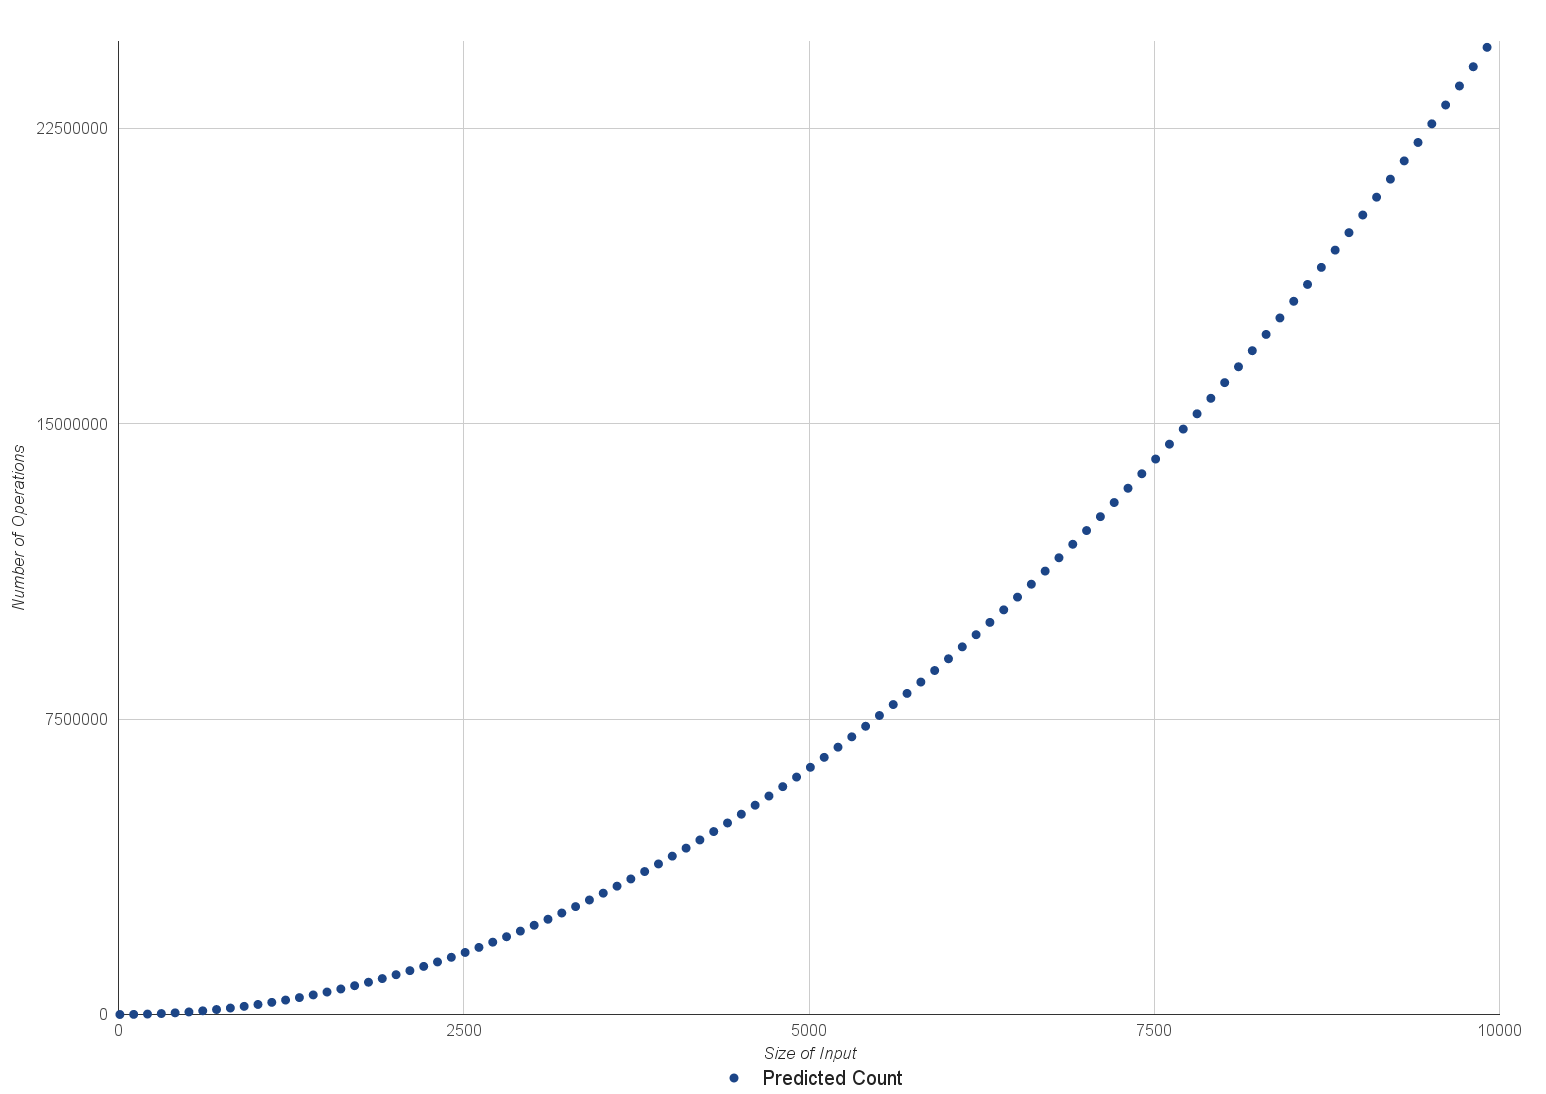
\includegraphics[scale=0.25]{predicted-count}\\[.1cm]
	\caption{\label{predicted-count}The blue circles are the count that represents the hypothesised number of operations given the size of the input  ($\frac{n^2}{4}$).}
\end{figure}
\newpage


\section{Average Basic Operations}
\begin{figure}[h]
	\centering
	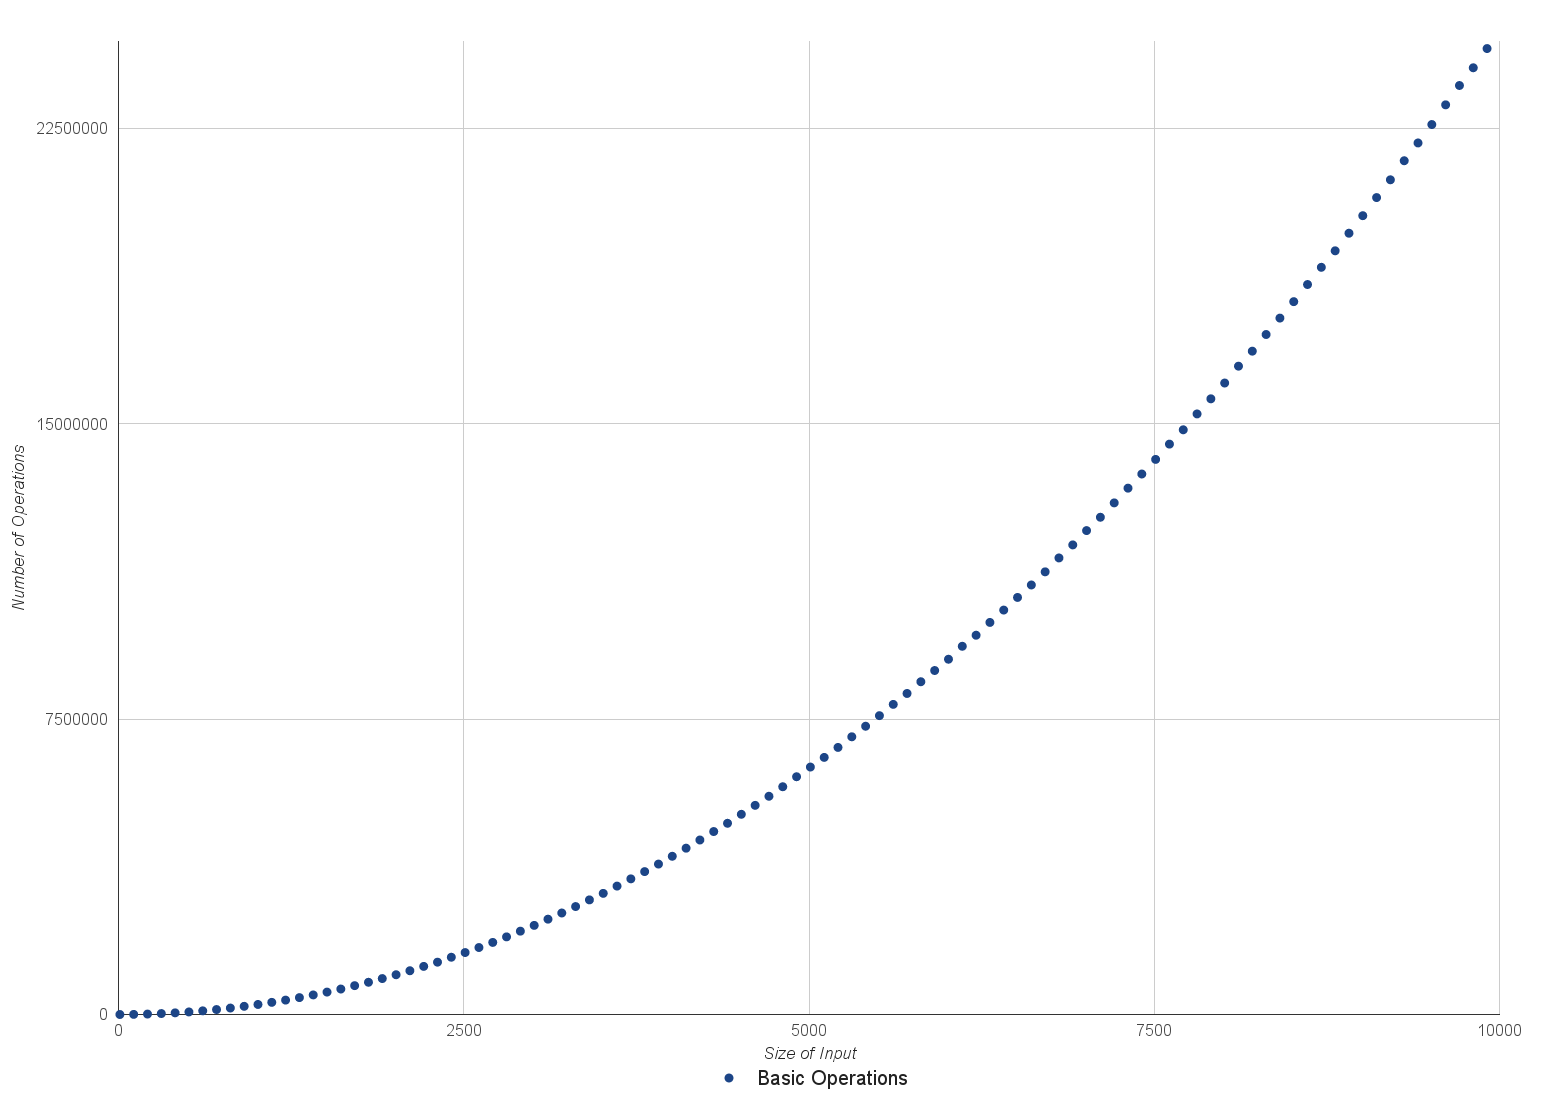
\includegraphics[scale=0.2]{AverageBasicOperations}\\[.1cm]
	\caption{\label{AverageBasicOperations} Each blue circle represents the average amount of basic operations it took over 100 iterations to sort an array, where the size of said array can be seen on the horizontal axis.}
\end{figure}

\newpage

\section{Average Time}
\begin{figure}[h]
	\centering
	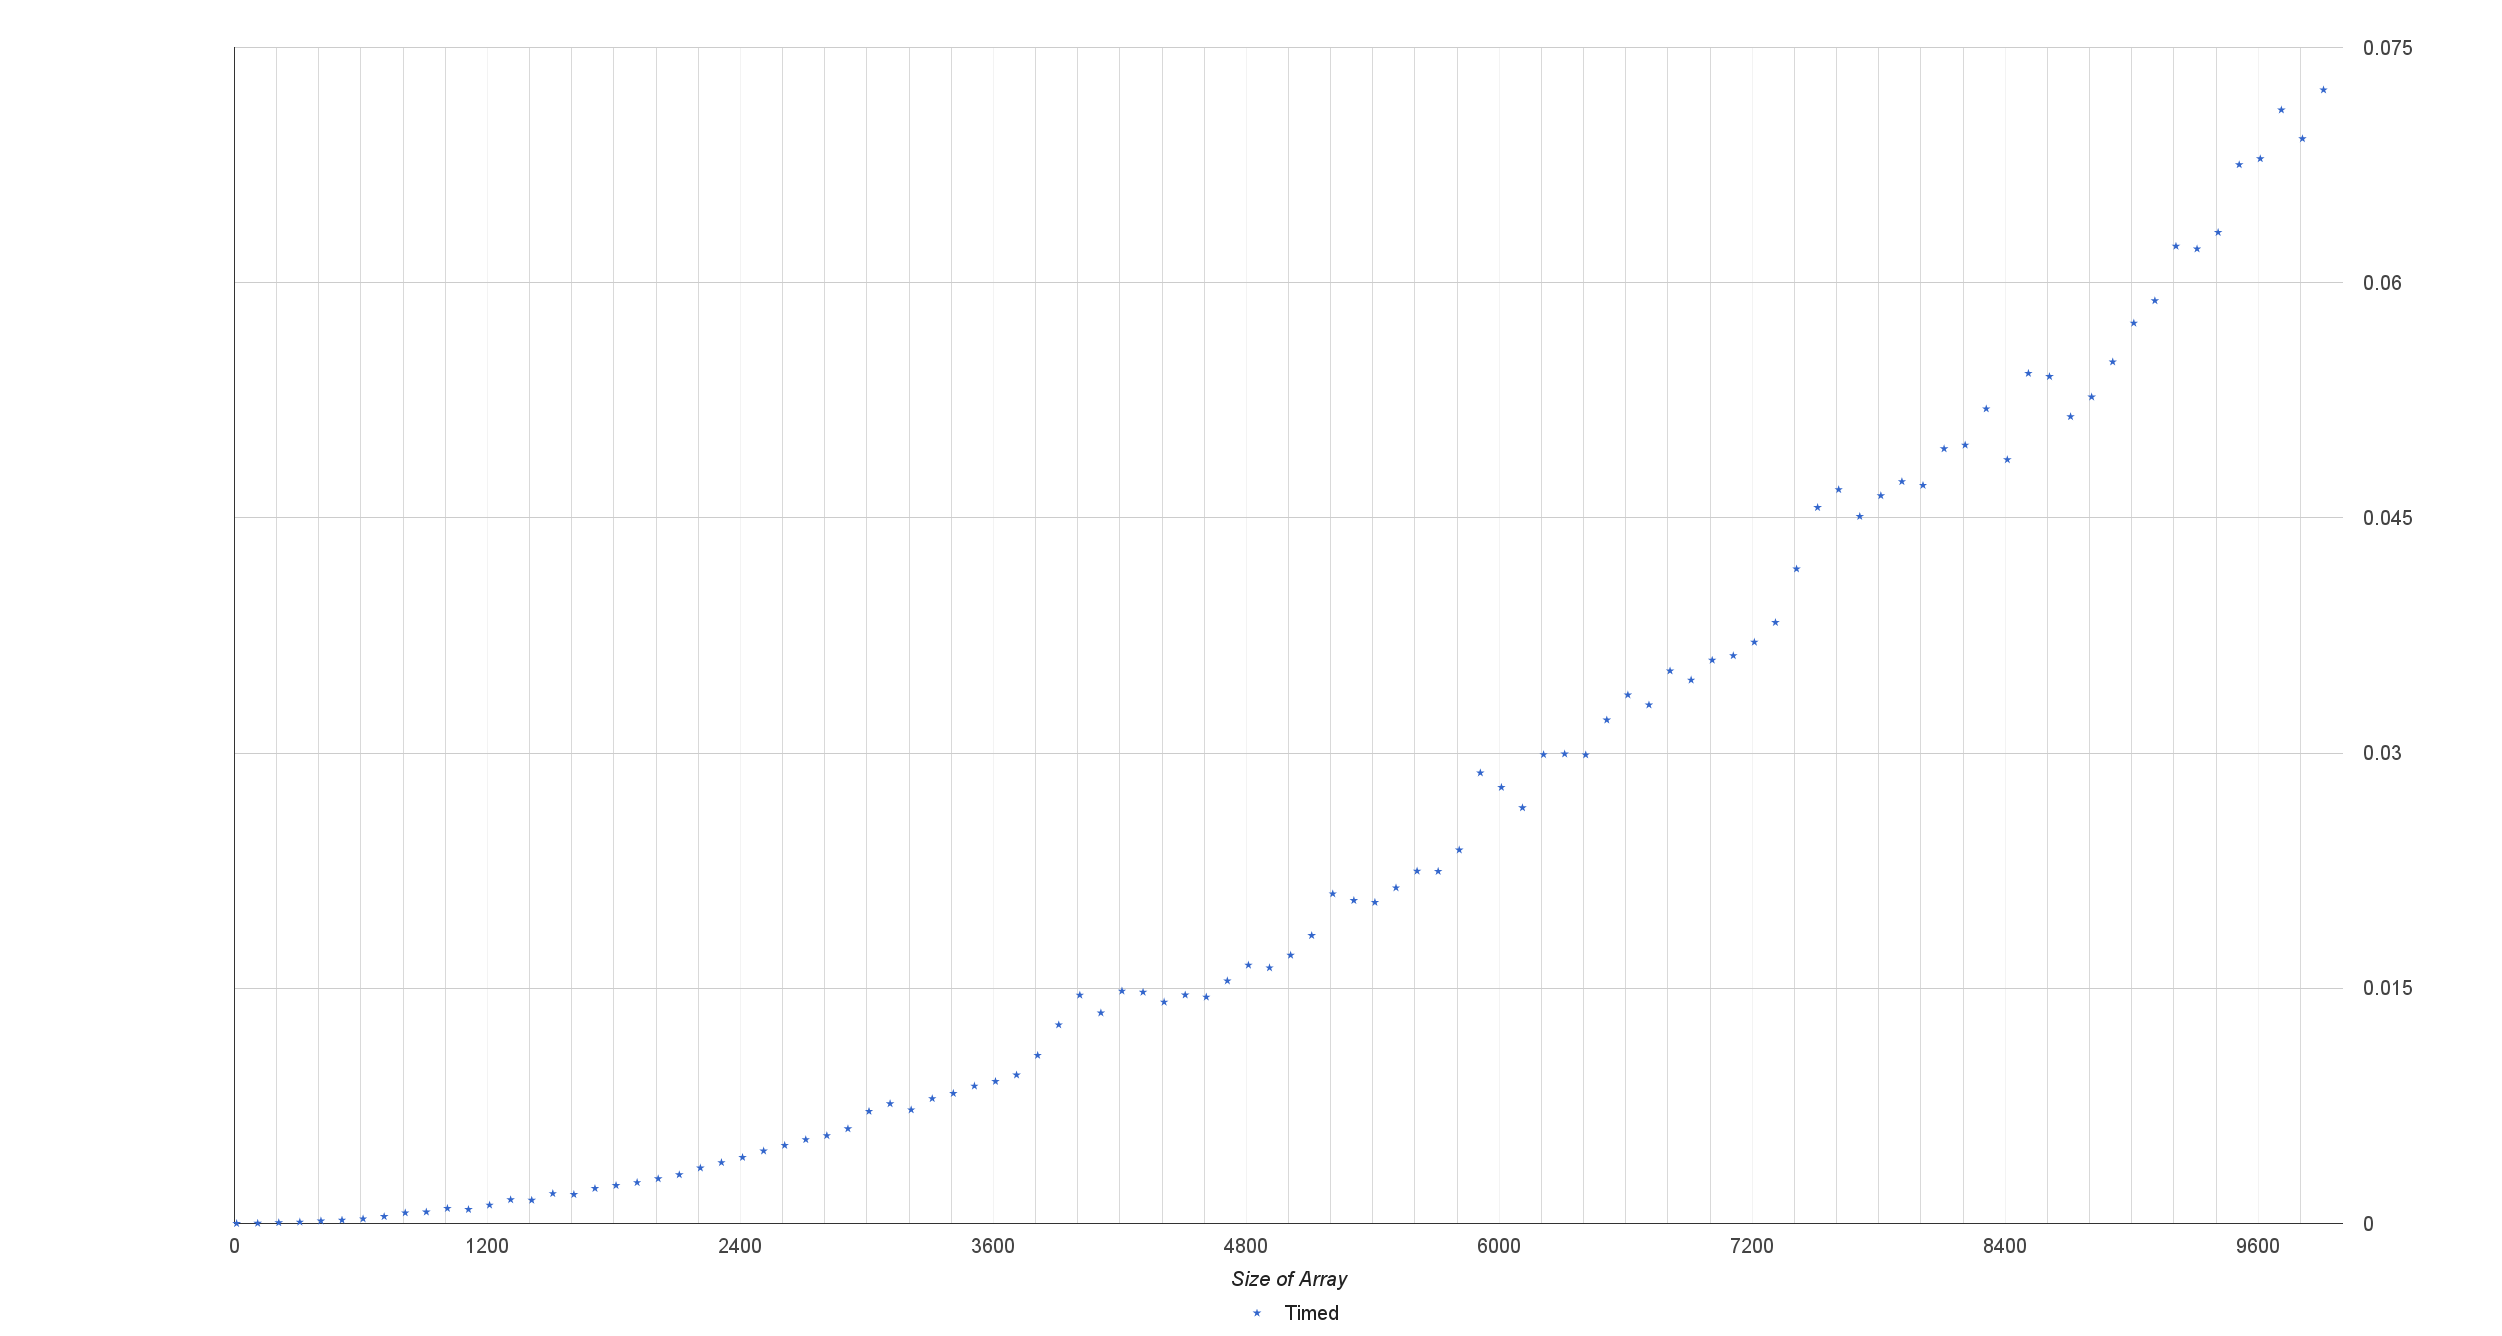
\includegraphics[scale=0.15]{average-time}\\[.1cm]
	\caption{\label{average-time}Each blue dot represents the average time it took over 100 iterations to sort an array, where the size of said array can be seen on the horizontal axis.}
\end{figure}

\newpage

\section{Average Time vs Size of Array}
\begin{figure}[h]
	\centering
	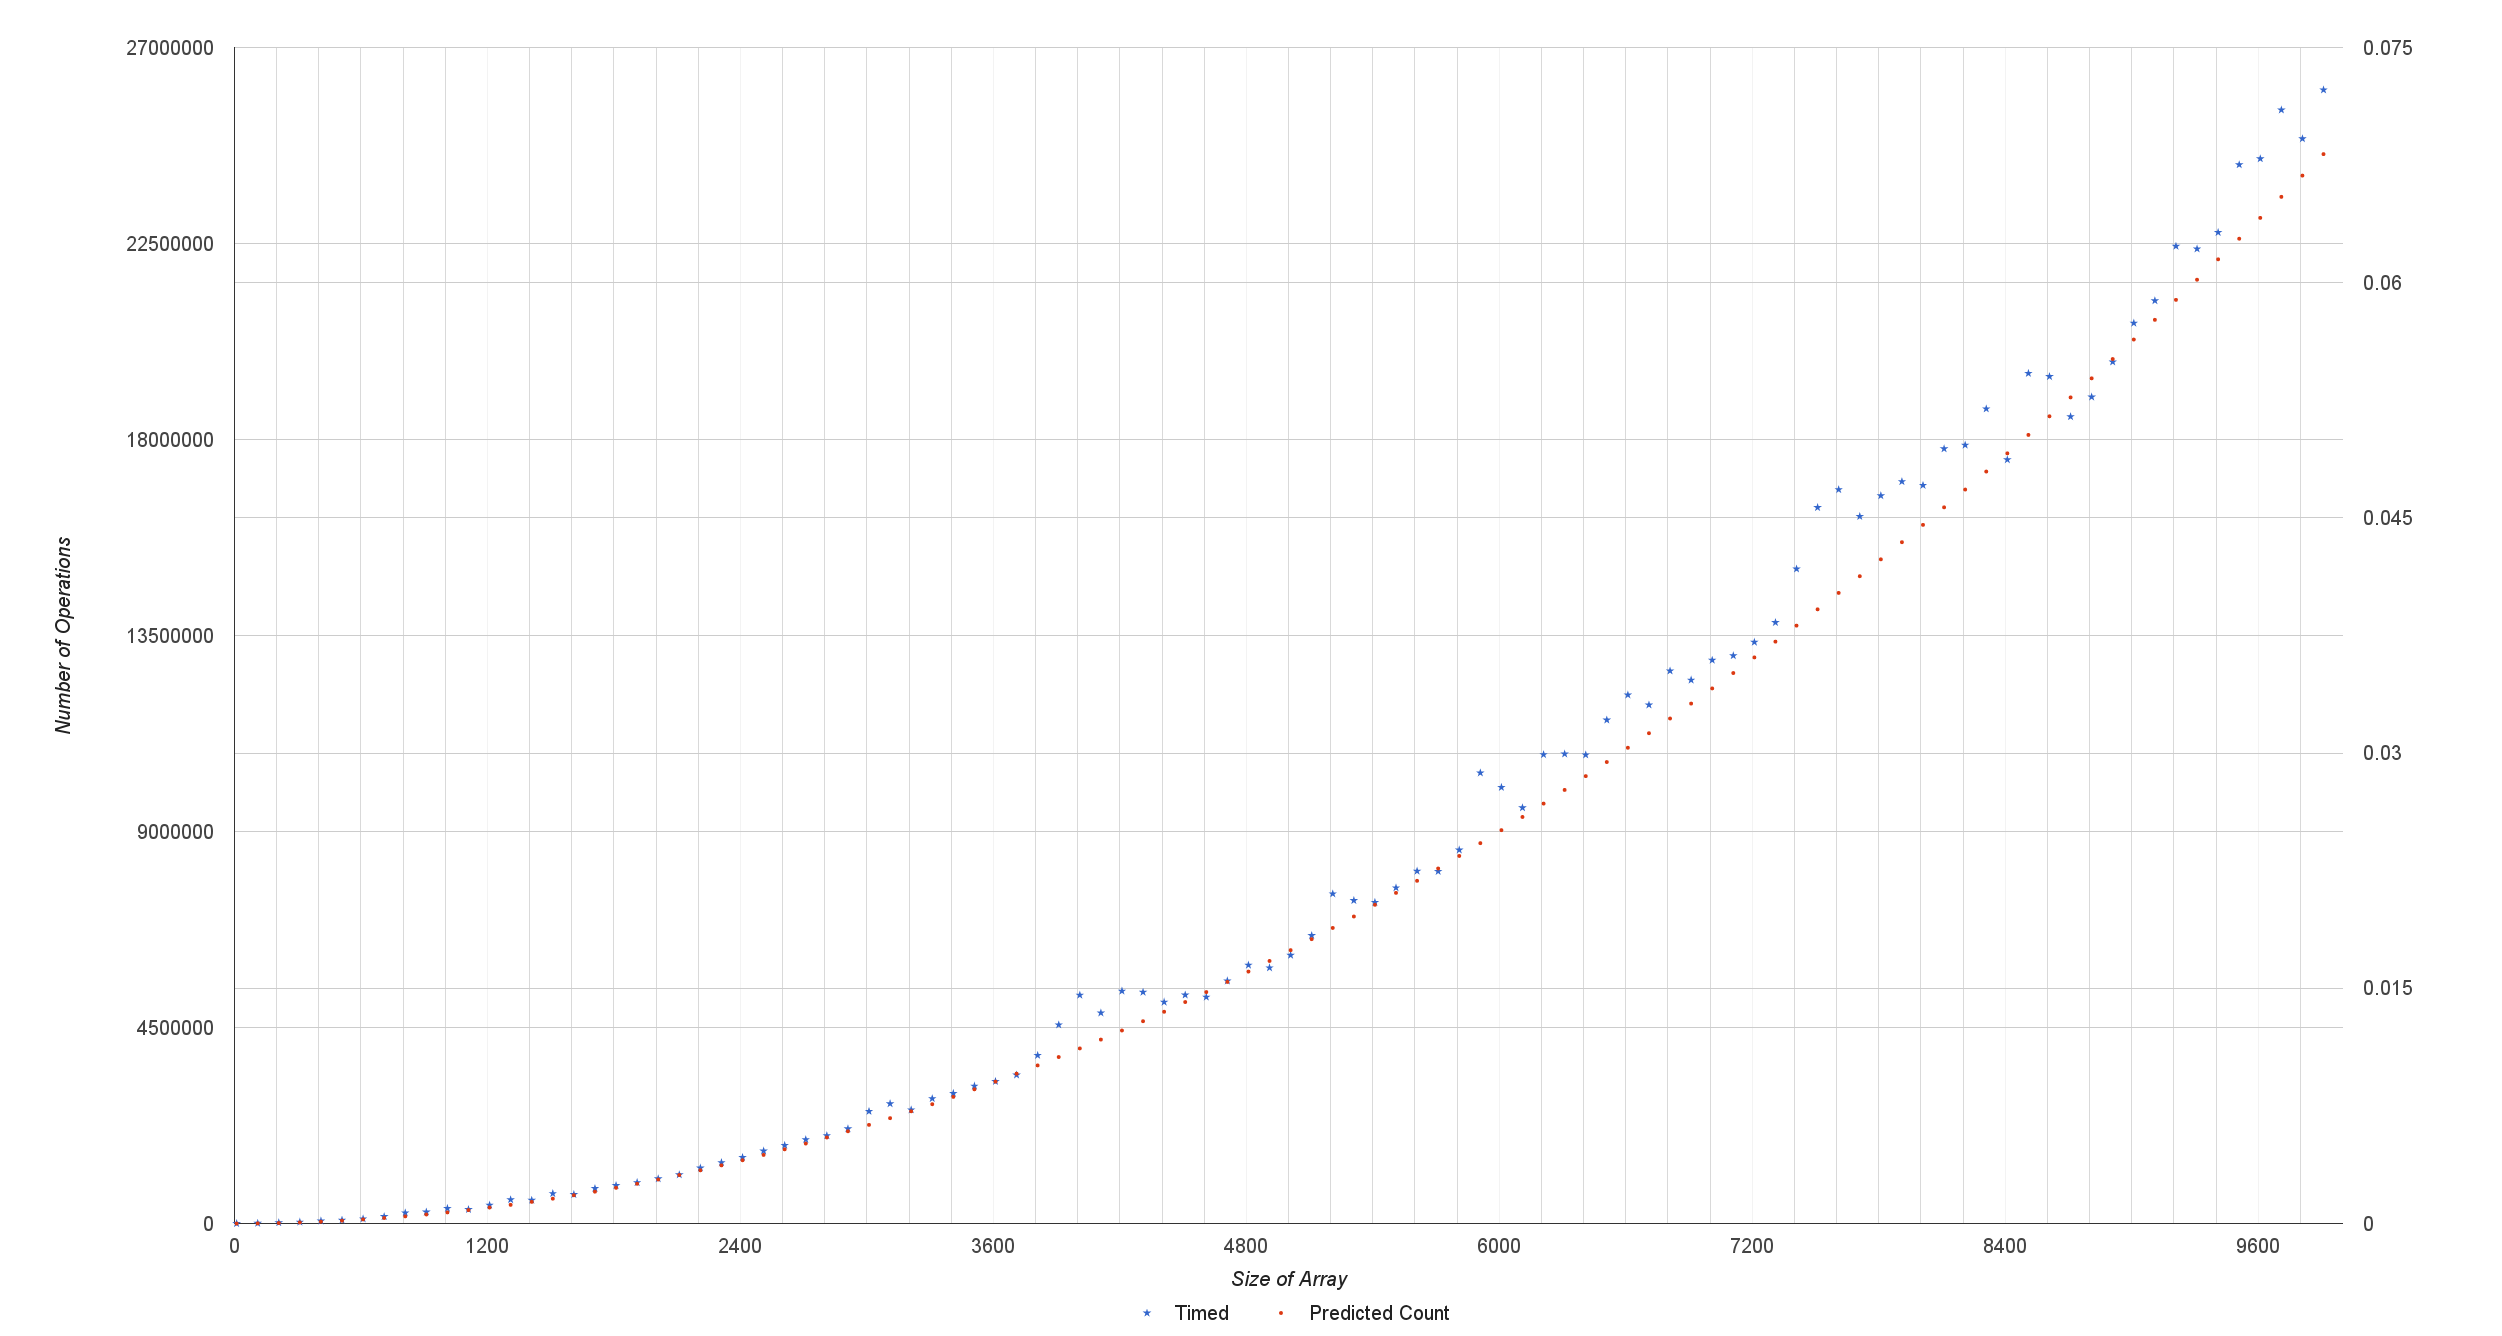
\includegraphics[scale=0.15]{average-time-vs-size-of-array}
	\caption{\label{average-time-vs-size-of-array}  Each blue star represents the average time it took over 100 iterations to sort an array, where the size of said array can be seen on the horizontal axis. The red circles are the count that represents the hypothesised number of operations given the size of the input ($\frac{n^2}{4}$).}
\end{figure}

\newpage


\section{Average Basic Operations Vs Predicted Count}
\begin{figure}[h]
	\centering
	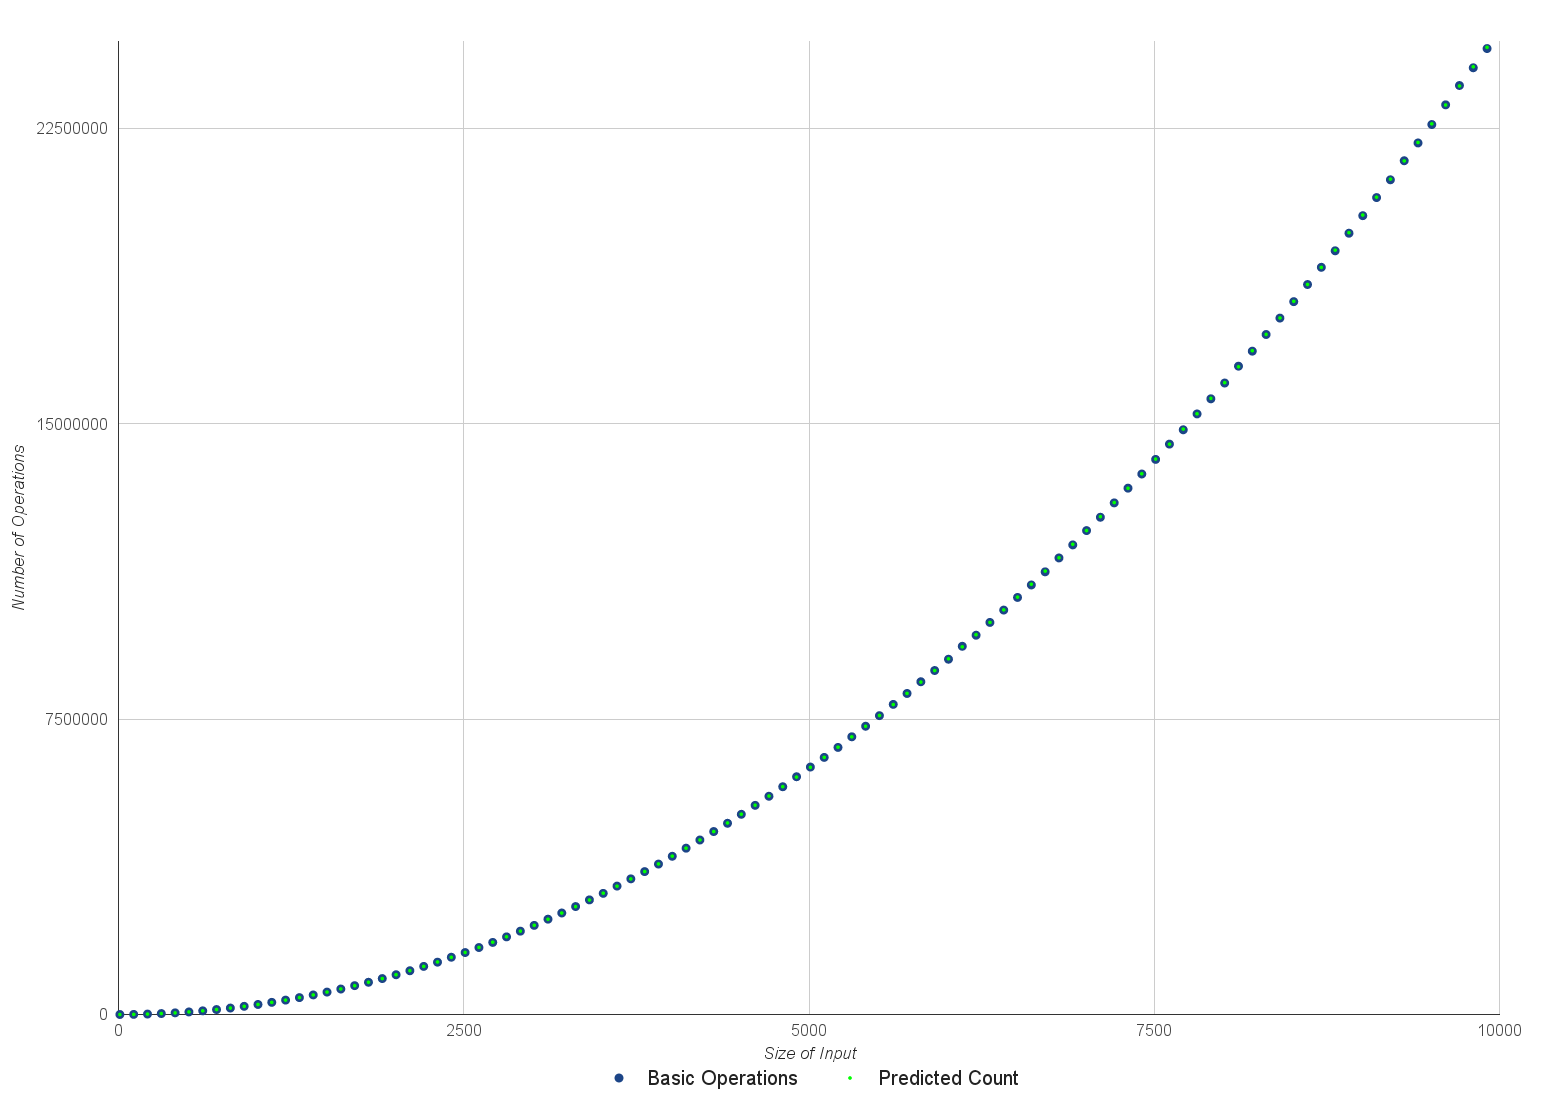
\includegraphics[scale=0.2]{AverageBasicOperationsVAssumedCount}\\[.1cm]
	\caption{\label{AverageBasicOperationsVAssumedCount} Each blue circle represents the average amount of basic operations it took over 100 iterations to sort an array, where the size of said array can be seen on the horizontal axis. The green circles which are inside of the blue circles represent  the count that represents the hypothesised number of operations given the size of the input  ($\frac{n^2}{4}$).}
\end{figure}

\newpage

\section{Total Basic Operations vs Size of Input}
\begin{figure}[h]
	\centering
	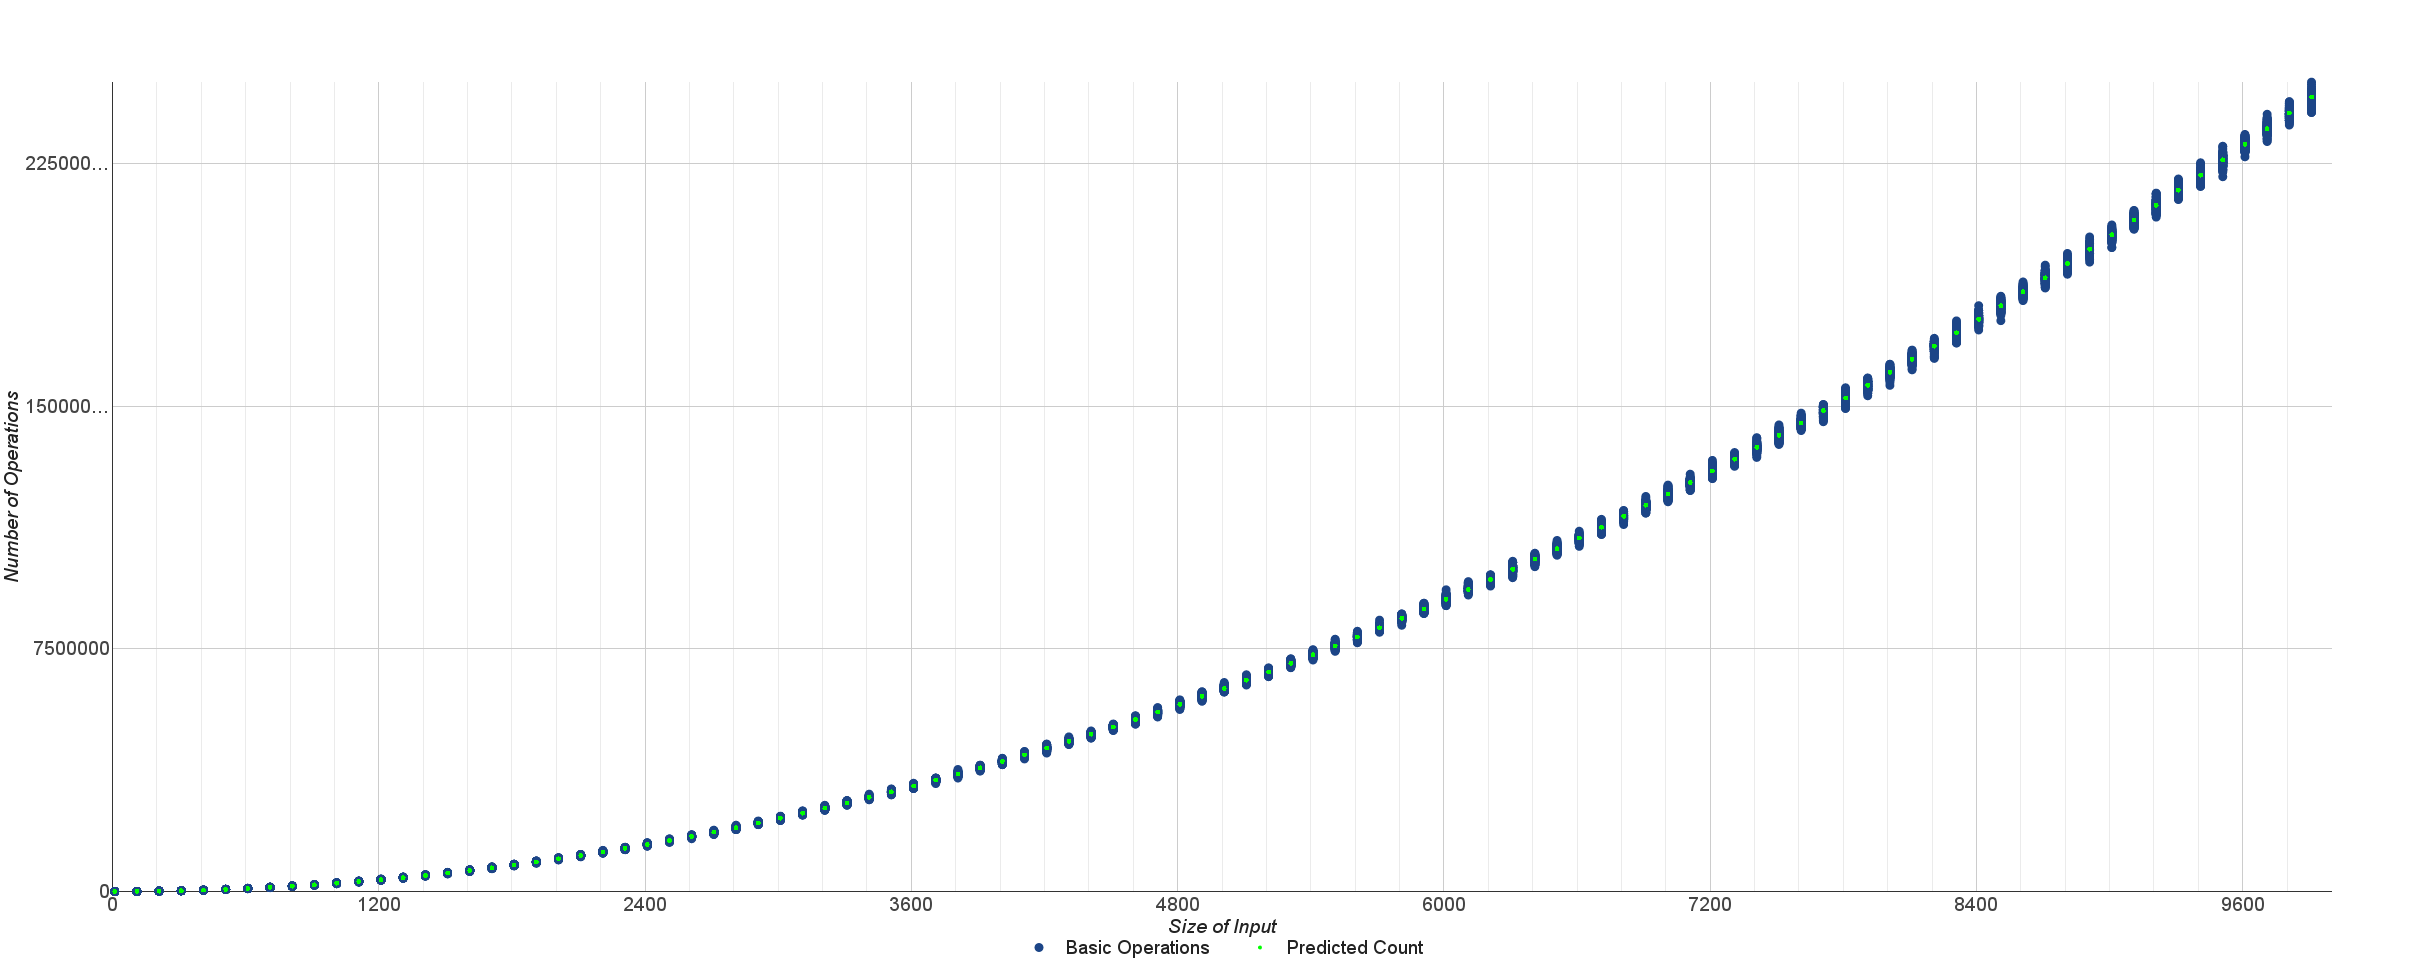
\includegraphics[scale=.15]{TotalOperationsVsHypothAmount}\\[.1cm]
	\caption{\label{total-basic-operations-v-size-of-input} The stark green circles are the count that represents the predicted number of operations given the size of the input which is a the graphical form of $\frac{n^2}{4}$. The blue circles, almost indistinguishable from being a blue line, are points making up every amount of basic operations that was completed at a given size of input. On this graph there are 100 points per Size of input so what is truly being represented here is the range of values for the experiment results.}
\end{figure}

\newpage

\end{appendices}
\end{document}
